\subsection{A gauge-invariant gap with unequal plaquette couplings}
\label{cl:sec:unequal}

Here the temporal plaquettes have coefficient $b\ge0$ and the spatial
plaquettes coefficient $\lambda\ge0$, both multiplying the normalized
real trace $x_p$. The two coefficients can be varied independently.
We estimate the partition functions themselves, including the spatial
plaquette weights. The result holds in a strong electric coupling regime.
For the relation of strong-coupling expansions to the spectrum see
\cite{Sei82,OSei78}. All spatial boundary conditions in this subsection
are periodic, with periods at least four, and $V$ is the number of sites.

Write $k_b(g)=e^{b x(g)}/\int e^{b x}\,dg$, where Haar measure has mass
one. Choose a positive integer $h$ with
$\|k_b^{*h}-1\|_\infty\le\eta$. Put
\[
 a_0=\frac{1}{2e^2\,80^2},\qquad
 A=\max\{\eta,\,(e^{h\lambda}-1)(1+\eta)^4\}.
\]
\begin{theorem}[Unequal-coupling Wilson partition ratio]\label{cl:thm:unequal-gap}
If $A\le a_0$ and $T=mh$ with integer $m\ge8$, then the ordinary
gauge-projected Wilson partition functions on the same spatial box satisfy
\[
 1\ \ge\ \frac{Z(2T)}{Z(T)^2}\ \ge\ \exp[-48Vm\,e^{-m/4}].
\]
The physical transfer matrix has excited-to-vacuum eigenvalue ratio
at most $e^{-1/(4h)}$, uniformly in spatial volume. For $\SU(2)$ one
may take $h=\lceil18(1+2b/3)\rceil$ and $0\le h\lambda\le10^{-6}$
at every $b$. For each fixed compact connected matrix group, the same
conclusions hold with an explicit $h=O_G((1+b)^2)$ specified below.
\end{theorem}

\begin{figure}[htbp]
\centering
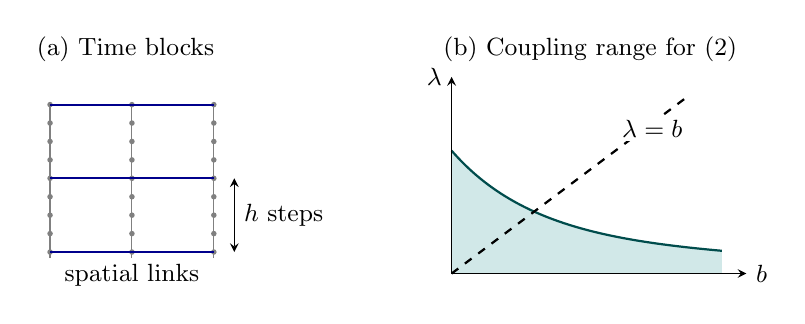
\begin{tikzpicture}[x=1.04cm,y=.78cm,>=stealth,font=\small]
\node[anchor=west] at (-.28,3.65) {(a) Time blocks};
\foreach \x in {0,1,2} {
  \draw[gray] (\x,.25)--(\x,2.8);
  \foreach \y in {.35,.65,.95,1.25,1.55,1.85,2.15,2.45,2.75}
    \fill[gray] (\x,\y) circle(1pt);}
\draw[thick,blue!55!black] (0,.35)--(2,.35) (0,1.55)--(2,1.55)
  (0,2.75)--(2,2.75);
\draw[<->] (2.25,.35)--(2.25,1.55) node[midway,right] {$h$ steps};
\node at (1,-.03) {spatial links};
\begin{scope}[xshift=5.1cm]
\node[anchor=west] at (-.22,3.65) {(b) Coupling range for $\SU(2)$};
\fill[teal!18] (0,0)--(0,2) .. controls (.75,.85) and (1.8,.55) ..
 (3.3,.37)--(3.3,0)--cycle;
\draw[thick,teal!60!black] (0,2) .. controls (.75,.85) and (1.8,.55) ..
 (3.3,.37);
\draw[thick,dashed] (0,0)--(2.9,2.9);
\node[fill=white,inner sep=1pt] at (2.45,2.35) {$\lambda=b$};
\draw[->] (0,0)--(3.6,0) node[right] {$b$};
\draw[->] (0,0)--(0,3.2) node[left] {$\lambda$};
\end{scope}
\end{tikzpicture}
\caption{In a time block the endpoint fields remain integrated. The
shaded region sketches the sufficient bound $h(b)\lambda\le10^{-6}$;
the axes are schematic. The isotropic ray leaves this region as $b$
increases.}\label{cl:fig:unequal}
\end{figure}

\begin{proof}
First take temporal gauge before applying the vertex gauge projection.
Use the normalized kinetic kernel $\prod_e k_b(Q_e^{-1}Q'_e)$ and the
full spatial action. This normalization multiplies a time-$T$ partition
function by a scalar exponential in $T$ and cancels from the ratio.
Denote the resulting trace by $Z^0(T)$. In its periodic path integral
group the time steps into $m$ slabs of length $h$. Include the spatial
action on slices $jh$ through $(j+1)h-1$ in slab $j$. For each spatial
plaquette $p$ in that slab expand its weight as $1+v_{p,j}$ with
\[
 v_{p,j}=\exp\!\left(\lambda\sum_{r=0}^{h-1}x_p(Q_{jh+r})\right)-1,
 \qquad |v_{p,j}|\le e^{h\lambda}-1.
\]
Call a selected term of this kind a plaquette mark. A spatial edge
traced through one slab is a column. Given the end values of all
columns, integrate the internal variables of every column touched by
a plaquette mark, with the full kinetic weight. All insertions sharing
a column are integrated together. After bounding each insertion in
absolute value, each touched column costs at most $1+\eta$, its
unrestricted end-to-end kernel bound. Each untouched column integrates
exactly to $1+u$, where $u=k_b^{*h}(Q_e^{-1}Q'_e)-1$ and $|u|\le\eta$.
Expanding these factors introduces a second kind of mark, a column
mark. A column mark is forbidden in a column already touched by a
plaquette mark of that slab.

Join two marks if their supports share an endpoint link variable.
A plaquette mark has eight such variables and a column mark has two.
An endpoint belongs to at most ten marks, since its spatial edge belongs
to four plaquettes in each adjoining slab and to one column in each.
The closed neighbourhood of a mark has size at most $80$. Disjoint
connected components use disjoint integration variables, including the
end values, which are integrated against product Haar measure. Thus
$Z^0(T)$ is exactly the partition function of mutually compatible
polymers. A polymer $\gamma$ is a nonempty connected set of marks;
its activity $w(\gamma)$ is its integrated weight, zero for a forbidden
choice. Two polymers are incompatible if their marks overlap or are
adjacent. There are at most four touched columns per plaquette mark.
It follows for the actual integrated activities that
$|w(\gamma)|\le A^{|\gamma|}$.

We give the constants for the log expansion. A connected set of size
$s$ containing a specified mark admits a depth-first traversal of
$2s-2$ steps. There are at most $80^{2s-2}$ possible traversals. Hence
\[
 \sum_{\gamma\ni v}|w(\gamma)|e^{2|\gamma|}
 \le \frac{Ae^2}{1-80^2Ae^2}\le 1/80^2
\]
at any mark $v$. Summing over the closed neighbours of a polymer meets
the Koteck\'y--Preiss criterion \cite{KP86} with size $|\gamma|$
and enlarged activities $|w(\gamma)|e^{|\gamma|}$. In particular the
sum of absolute log-cluster coefficients containing a designated
occurrence of a given polymer is at most
$|w(\gamma)|e^{2|\gamma|}$ after weighting each cluster by $e^s$,
where $s$ counts all its marks with polymer multiplicity. This is the
rooted bound in the criterion, with the root activity included.
Thus the total absolute contribution of clusters of size at least
$m/4$ on the $m$-slab torus is at most $6Vm\,e^{-m/4}$: there are
$3V$ possible marks of each type per slab, and counting a cluster
at several roots only increases the upper bound.

It remains to compare the small clusters. Distribute each cluster
coefficient equally over its $s$ mark occurrences. From a rooted mark
all other marks are reached in at most $s-1$ adjacency steps; one
step changes the slab coordinate by at most one. For $s<m/4$ the
interval of lifted slab coordinates about the root, including adjacent
endpoints, has length less than $m$. Lifting therefore preserves all
identifications, incompatibilities, activities and multiplicities.
Equivalently every such rooted pattern at period $m$ has two rooted
lifts at period $2m$ and every small rooted pattern upstairs projects
back. Their contributions cancel in $2\log Z^0(T)-\log Z^0(2T)$.
Applying the tail bound with the common cutoff $m/4$ at both periods
gives
\[
 0\le \psi^0(T)=2\log Z^0(T)-\log Z^0(2T)
 \le 24Vm\,e^{-m/4}.
\]
Positivity of the transfer spectrum gives the first inequality.

For clarity, the propagation in this argument is in time only;
permuting the time and space directions would change the action.
The strictly positive temporal-gauge kernel has a unique positive
vacuum, invariant under the commuting gauge action. Its operator is
positive by the same power-series argument as in
Theorem~\ref{cl:thm:charged-gap}. If $D^0(T)$ sums all excited normalized
eigenvalues to the power $T$, positivity gives
$\log(1+D^0(T))\le\psi^0(T)$: the denominator of the purity ratio
is bounded by $1+D^0(T)$. The physical projection retains the vacuum
and a subset of the excited spectrum. Consequently
$0\le2\log Z(T)-\log Z(2T)\le2\log(1+D^0(T))\le2\psi^0(T)$.
At fixed $V$, each excited ratio $r$ also satisfies
$r^{mh}\le D^0(mh)\le\exp(24Vm e^{-m/4})-1$. Taking $(mh)$th
roots as $m\to\infty$ gives the claimed volume-independent gap.

For $\SU(2)$ the character calculation in Theorem~\ref{cl:thm:row-law}
applies to the free kinetic column with parameter $s=b$. Thus
$\eta\le(1+u)/(1-u)^3-1$ with $u=[2b/(3+2b)]^h\le e^{-18}$ for
the stated choice of $h$. Here $\eta\le6e^{-18}<10^{-6}$.
For another fixed connected group, use Lemma~\ref{cl:lem:general-row}
for $h$ steps of the single-link law, whose exponent also obeys the
six-staple derivative and supremum bounds used there. Its parameter
$q_G$ gives $\eta\le e^{-20}$ on taking
$h=2+\lceil(12b+20)/(-\log q_G)\rceil$. This is $O_G((1+b)^2)$.
In either case $(e^{h\lambda}-1)(1+\eta)^4<4\cdot10^{-6}<a_0$
when $0\le h\lambda\le10^{-6}$.
\end{proof}

For example on $n=24T$ this lower bound on the ratio tends to one
whenever $Vm e^{-m/4}\to0$. It therefore crosses $97/169$ in that
range for the actual unequal-coupling model. The isotropic trajectory
requires $\lambda=b\to\infty$. Even rescaling a plaquette mark by the
best constant cannot make its uniform size small there: its weight
ranges from $e^{-h\lambda}$ to $e^{h\lambda}$ for $\SU(2)$, since
the four links may be held constant through the slab with plaquette
product $-I$ or $I$. The minimum of $\sup|w/c-1|$ over $c>0$ is
$\tanh(h\lambda)$. This locates the failure of this absolute expansion
before it could give an isotropic bound.

\subsection{Continuous time and a gauge-invariant excitation}
\label{cl:sec:electric-hamiltonian}
Keep the spatial lattice fixed and let the temporal spacing be $t$.
For $\SU(2)$ on the unit three-sphere put $b=B/t$ and $\lambda=\kappa t$,
where $B>0$ and $0<12B\kappa<10^{-6}$. Write $\Delta_e$ for the
Laplace operator of the unit sphere on link $e$. In this normalization
the Kogut--Susskind lattice Hamiltonian \cite{KS75}, shifted by a constant, is
\[
 H=\frac1{2B}\sum_e(-\Delta_e)+\kappa\sum_p(1-x_p).
\]
It acts on the tensor-product link space; gauge-invariant vectors form
the physical subspace.

\begin{theorem}[A two-sided physical lattice bound]\label{cl:thm:electric-packet}
On every periodic spatial cube of side at least four, let $E_0,E_1$
be the lowest and next physical energies of $H$. Then
\[
 \frac{1}{48B}\le E_1-E_0\le\frac{10}{B}.
\]
For any elementary spatial plaquette, the variance of $f=x_p$ in the
unit vacuum $\Omega$ is at least $1/5$. Its centered, contact-normalized
two-point function at time $\tau\ge0$ lies between
$e^{-10\tau/B}$ and $e^{-\tau/(48B)}$, uniformly in spatial volume.
\end{theorem}
\begin{proof}
We first justify passage to continuous time at fixed volume. Put
$W=\kappa\sum_p(1-x_p)$, $D_t=e^{-tW/2}$ and let $C_t$ be the product
of the normalized free single-link kinetic convolutions. The operator
$K_t=D_tC_tD_t$ differs from the normalized Wilson transfer of the
previous theorem only by a scalar. Write $H_{0,t}=(I-C_t)/t$ and
$H_0=\sum_e(-\Delta_e)/(2B)$. For each fixed representation of
dimension $\ell+1$ the one-link kinetic eigenvalue is
$1-t\ell(\ell+2)/(2B)+o_\ell(t)$. Indeed the normalized character at
angle $\theta$ is $1-\ell(\ell+2)\theta^2/6+O_\ell(\theta^4)$.
Under the density proportional to $e^{b\cos\theta}\sin^2\theta$,
the substitution $r=\sqrt b\,\theta$ gives
$b\,\mathbb E\theta^2\to3$ and $\mathbb E\theta^4=O(b^{-2})$.
Dominated convergence uses $1-\cos\theta\ge2\theta^2/\pi^2$ and
$|\sin\theta|\le\theta$ on $[0,\pi]$. The limiting radial Gaussian
has density proportional to $r^2e^{-r^2/2}$.

The free resolvents converge in operator norm. On modes of bounded
total degree $\sum_e\ell_e$ this follows by multiplication of the
single-link eigenvalues on a finite-dimensional space. On total
degree at least $J$ the eigenvalue of $C_t$ is at most
$[2b/(3+2b)]^J$ by the Bessel-ratio bound. Thus the lower bound for
$H_{0,t}$ on that tail tends, for fixed $J$, to $3J/(2B)$ as $t\to0$.
The limiting $H_0$ has the same lower bound there, since
$\ell(\ell+2)\ge3\ell$. Letting $J\to\infty$ proves norm convergence
of $(H_{0,t}+c)^{-1}$ for every $c>0$.

For $H_t=(I-K_t)/t$ one has the exact factorization
\[
 H_t+c=D_t\,[\,H_{0,t}+c+(t^{-1}+c)(D_t^{-2}-I)\,]\,D_t .
\]
The additional bounded operator inside brackets tends to $W$ in norm.
Taking $c>2\|W\|+1$, the Neumann series for the inverse is uniformly
convergent for small $t$. Since $D_t\to I$, the resolvents of $H_t$
converge in norm to those of $H_0+W$ at $-c$. Everything commutes
with the gauge projection. The limiting resolvent is compact, and
the top two eigenvalues of the physical resolvents converge by the
min--max principle. In fact the essential point of the finite-step
resolvent is $(c+1/t)^{-1}$, tending to zero, because $K_t$ is compact.
Thus with $\lambda_0(t),\lambda_1(t)$ the top two physical eigenvalues
of $K_t$, $(1-\lambda_j(t))/t\to E_j$ for $j=0,1$. In particular
$\lambda_0(t)\to1$. The row length in
Theorem~\ref{cl:thm:unequal-gap} satisfies $th\to12B$, so that
$h\lambda<10^{-6}$ eventually. Taking the limit of
$\lambda_0(t)(1-e^{-1/(4h)})/t$ gives the claimed lower bound.

The compact connected link manifold has a strictly positive heat
kernel. A bounded real potential preserves positivity improving by
the heat-kernel path formula. Hence $H$ has a unique positive unit
vacuum; it is invariant under the gauges, spatial translations and
cubic rotations. The constant trial function gives $E_0\le3V\kappa$
because each Haar plaquette has mean zero. Since $W\ge0$ and the
$3V$ links are equivalent, $\|\nabla_e\Omega\|_2^2\le2B\kappa$
for each $e$. (Reversing a link is an isometry.)

Fix an edge $e$ of the plaquette and let $P_e$ average over this link
alone. The first nonzero eigenvalue of $-\Delta$ on the unit $S^3$ is
three. Hence $\epsilon=\|\Omega-P_e\Omega\|_2\le\sqrt{2B\kappa/3}<1/50$.
Haar integration in that edge gives $P_e f=0$, $P_e f^2=1/4$;
the latter is the second moment of one coordinate of a uniform
unit quaternion. For a multiplier of norm at most one its quadratic
forms at $\Omega$ and $P_e\Omega$ differ by at most $2\epsilon$.
As $\|P_e\Omega\|^2=1-\epsilon^2$, this yields
\[
 \operatorname{Var}_\Omega f\ge
 \frac14-2\epsilon-\frac{17}{4}\epsilon^2\ge\frac15 .
\]
Write $F=(f-\langle f\rangle_\Omega)\Omega$. It is a physical vector
orthogonal to the vacuum. Testing the ground-state equation against
$(f-\langle f\rangle_\Omega)^2\Omega$ and integrating by parts gives
\[
 \langle F,(H-E_0)F\rangle
 =\frac{1}{2B}\sum_e\int |\nabla_e f|^2|\Omega|^2\le \frac2B .
\]
Only four links enter, and on each $f$ is a coordinate on the unit
sphere composed with an isometry, with gradient length at most one.
Dividing by $\|F\|^2$ and applying the variational principle gives
the upper bound on $E_1-E_0$. For the spectral probability measure of
$F/\|F\|$, Jensen's inequality for $E\mapsto e^{-\tau E}$ gives the
lower two-point bound, and the lower spectral edge gives the upper one.
\end{proof}
The lattice spacing in the three spatial directions has been held fixed.
The estimates construct a finite-energy plaquette excitation in this
continuous-time lattice theory. They give no estimate along the
four-dimensional isotropic asymptotic-freedom trajectory.
